\documentclass{sig-alternate}

\usepackage[utf8]{inputenc}
\usepackage{enumitem}
\usepackage[hyphens]{url}
\usepackage[pdftex,urlcolor=black,colorlinks=true,linkcolor=black,citecolor=black]{hyperref}

\newcommand{\superscript}[1]{\ensuremath{^{\textrm{#1}}}}

% listings and Verbatim environment
\usepackage[usenames,dvipsnames,svgnames,table]{xcolor}
\usepackage{fancyvrb}
\usepackage{relsize}
\usepackage{listings}
\usepackage{verbatim}
\newcommand{\defaultlistingsize}{\fontsize{8pt}{9.5pt}}
\newcommand{\inlinelistingsize}{\fontsize{8pt}{11pt}}
\newcommand{\smalllistingsize}{\fontsize{7.5pt}{9.5pt}}
\newcommand{\listingsize}{\defaultlistingsize}
\RecustomVerbatimCommand{\Verb}{Verb}{fontsize=\inlinelistingsize}
\RecustomVerbatimEnvironment{Verbatim}{Verbatim}{fontsize=\defaultlistingsize}
\lstset{frame=lines,captionpos=b,numberbychapter=false,escapechar=§,
        aboveskip=2em,belowskip=1em,abovecaptionskip=0.5em,belowcaptionskip=0.5em,
        framexbottommargin=-1em,basicstyle=\ttfamily\listingsize\selectfont}

% use Courier from this point onward
\let\oldttdefault\ttdefault
\renewcommand{\ttdefault}{pcr}
\let\oldurl\url
\renewcommand{\url}[1]{\inlinelistingsize\oldurl{#1}}

\lstdefinelanguage{JavaScript}{
  keywords={console, log, addEventListener, onmessage, alert, push, typeof, new, true, false, catch, function, return, null, catch, switch, var, if, in, while, do, else, case, break},
  keywordstyle=\bfseries,
  ndkeywords={class, export, boolean, throw, implements, import, this},
  ndkeywordstyle=\color{darkgray}\bfseries,
  identifierstyle=\color{Maroon},
  sensitive=false,
  comment=[l]{//},
  morecomment=[s]{/*}{*/},
  commentstyle=\color{ForestGreen},
  stringstyle=\color{Blue},
  morestring=[b]',
  morestring=[b]"
}

% linewrap symbol
\usepackage{color}
\definecolor{grey}{RGB}{130,130,130}
\newcommand{\linewrap}{\raisebox{-.6ex}{\textcolor{grey}{$\hookleftarrow$}}}

% todo macro
\usepackage{color}
\newcommand{\todo}[1]{\noindent\textcolor{red}{{\bf \{TODO}: #1{\bf \}}}}

\begin{document}
%
% --- Author Metadata here ---
\conferenceinfo{International World Wide Web Conference}{2014 Seoul, Korea}
\CopyrightYear{2014} % Allows default copyright year (20XX) to be over-ridden - IF NEED BE.
%\crdata{0-12345-67-8/90/01}  % Allows default copyright data (0-89791-88-6/97/05) to be over-ridden - IF NEED BE.
% --- End of Author Metadata ---

\title{Bots vs. Wikipedians, Anons vs. Logged-In Humans:\\ A~Global Study of Edit Activity on Wikipedia and Wikidata}

\numberofauthors{1}

\author{
% 1st. author
\alignauthor
Thomas Steiner\titlenote{Thomas Steiner's second affiliation is \emph{Université de Lyon, CNRS Université Lyon~1, LIRIS, UMR5205, F-69622}}\\
       \affaddr{Google Germany GmbH}\\
       \affaddr{ABC-Str.~19}\\
       \affaddr{20354 Hamburg, Germany}\\
       \email{tomac@google.com}
}

\maketitle
\begin{abstract}
Wikipedia is a~global crowdsourced encyclopedia
that at time of writing is available in 287 languages.
Wikidata is a~likewise global crowdsourced knowledge base
that provides shared facts to be used by Wikipedias.
In the context of this research, we have developed
an application capable of monitoring
realtime edit activity of all language versions
of Wikipedia and Wikidata.
This application allows us and others to easily analyze edits
in order to answer questions such as
``Bots \emph{vs.}\ Wikipedians, who edits more?'',
``Anonymous \emph{vs.}\ logged-in humans, who edits what?'',
or ``Who are the bots and what do they edit?''.
To the best of our knowledge,
this is the first time such analyses
were done for really \emph{all} Wikipedias%
---big and small---and for Wikidata.
For evaluation purposes, our application is available publicly at
\url{http://wikipedia-edits.herokuapp.com/},
its code has been open-sourced under the Apache~2.0 license.
\end{abstract}

\category{ToDo}{\todo{category}}{}

\terms{\todo{terms}}

\keywords{\todo{keywords}}

\section{Introduction}

\paragraph{How Wikipedia Came Into Life}

The fundamental shift from book-based encyclopedias
to CD-ROM-based encyclopedias
to finally Web-based encyclopedias
happened in the course of the 90ies
and started a~new era of freely and openly
available knowledge accessible to everybody.
The free online encyclopedia Wikipedia%
\footnote{Wikipedia: \url{http://www.wikipedia.org/}}~\cite{sanger05historywikipedia} was formally launched
on January 15, 2001 by Jimmy Wales
and Larry Sanger,
albeit the fundamental technology and the underlying concepts are older.
Wikipedia's direct predecessor was Nupedia~\cite{sanger05historywikipedia},
a~similarly free online encyclopedia,
however, that was exclusively edited by experts
following a~strict peer-review process.
Wikipedia's initial role was to serve
for collaborating on draft articles for Nupedia.
What happened in practice was that Wikipedia rapidly overtook Nupedia
as there was no peer-review burden
and at time of writing is now a~global project
available in 287 languages and overall more than 30 million articles.%
~\footnote{Wikipedia statistics: \url{http://stats.wikimedia.org/}}

\paragraph{International Expansion}

The international expansion began early on
in the project's existence,
with the first two non-English Wikipedias
being on March 16, 2001 the German and the Catalan ones,
followed briefly afterwards by (Romanized) Japanese.
What then followed was a~wave of new languages,
with French, Chinese, Dutch, Esperanto, Hebrew,
Italian, Portuguese, Russian, Spanish, Swedish,
Arabic, Hungarian, Afrikaans, Norwegian, and Serbian all being rolled out in the first year.

\paragraph{The First Wikipedia Bots}

Wikipedia bots are computer programs
with the purpose of automatically editing Wikipedia.
After occasional smaller-scale tests,
the first large-scale bot operation
was started in October 2002 by Derek Ramsey,%
\footnote{History of Wikipedia bots: \url{http://en.wikipedia.org/wiki/Wikipedia\%3AHistory_of_Wikipedia_bots}}
who created a~bot to add a~large number
of articles about United States towns
based on tabular information
stemming from U.S. census data.
The generated articles used a~uniform
text template, so that all articles
followed the same writing style.
Today, bots are not only used to generate articles,
but also to fight vandalism and spam,
to correct typographic errors,
to improve references, and many more automatable tasks.%
\footnote{Wikipedia bots by purpose: \url{http://en.wikipedia.org/wiki/Category:Wikipedia_bots_by_purpose}}

\paragraph{The Knowledge Base Wikidata}

As Wikipedia is a~truly global effort,
sharing non-language-dependent facts
like population figures centrally
in a~knowledge base makes a~lot of sense.
Wikidata\footnote{Wikidata: \url{http://www.wikidata.org/}}~\cite{vrandecic2012wikidata}
is a~free knowledge base that can be read
and edited by both humans and bots.
The knowledge base centralizes access to
and management of structured data,
such as references between Wikipedias
and statistical information that can be used in articles.
Controversial facts such as borders in conflict regions
can be added with multiple values with sources,
so that Wikipedia article can,
dependent on their standpoint, choose their source.

\section{Related Work}

The Wikimedia Foundation themselves provide regular
statistics for all Wikipedias~\cite{zachte2013wikipedia}
with ten or more articles and edits in the previous month,
as well as statistics for Wikidata~\cite{zachte2013wikidata}.
These statistics are based on recent database dump files
and contain a~note that \textit{``the lengthy dump process
(many weeks) means [that] a~delay in publishing these statistics
is always to be expected''}.
We accessed the statistics on December 13, 2013,
where the data was processed up until October 31, 2013.
Based upon the fact that these database dumps
of all Wikipedias are also publicly available,
in 2005 Voß~\cite{voss2005measuring} gave 
an overview on Wikipedia research
and analyzed articles, authors, edits, and links,
as well as content and quality.
A~similar study on Wikipedia research dating from 2006
has been conducted by Ayers~\cite{ayers2006researchingwikipedia}.
Unlike the methods described in%
~\cite{ayers2006researchingwikipedia,voss2005measuring,zachte2013wikidata,zachte2013wikipedia},
our approach works in realtime.
In~\cite{ciampaglia2010empiricalanalysis}, Ciampaglia and Vancheri
perform an empirical analysis of user participation
excluding bots in five large Wikipedias.
Adler \emph{et~al.}\ study in~\cite{adler2008measuringauthor}
various means to measure user contributions to Wikipedia.
As a~part of their study, they analyze bot editors
that, if they were included, created massive outliers
in the introduced measures.
In contrast to the approaches%
~\cite{adler2008measuringauthor,ciampaglia2010empiricalanalysis},
we do not exclude bots for our analysis,
but rather include them as equal citizens,
while at the same time still allowing for dynamically
disregarding them if need be.
Several tools provide processed page view statistics
based on database dumps, examples are
\emph{Wikipedia article traffic statistics}%
\footnote{Wikipedia article traffic statistics:
\url{http://stats.grok.se/}} by ``User:Henrik'',
\emph{Wikipedia article traffic statistics}%
\footnote{Wikipedia article traffic statistics:
\url{http://toolserver.org/~emw/wikistats/}} by ``User:Emw'',
or finally \emph{Wikipedia Page Views}%
\footnote{Wikipedia Page Views: \url{http://wikistats.ins.cwi.nl/}}
by Hannes Mühleisen.
We do not focus on page view statistics based on database dumps,
but realtime article edit statistics instead.
In~\cite{boukhelifa2010realtime}, Boukhelifa \emph{et~al.}\
classify statistics tools in the categories global and local.
According to this classification,
local tools focus on individual articles or users
and therefore require time-consuming on-the-fly computations.
In contrast,  global tools
show the evolution of aggregated data
for all Wikipedias,
but without acquiring realtime data.
According to this classification, our approach can be
classified as global, however, with realtime support.

\section{Implementation Details}

\paragraph{Wikipedia Recent Changes}

Whenever a~human or bot changes an article
of any of the 287 Wikipedias,%
\footnote{List of Wikipedias by size:
\url{http://meta.wikimedia.org/wiki/List_of_Wikipedias}}
a~change event gets communicated by a~chat bot
over Wikipedia's own Internet Relay Chat~(IRC) server (\url{irc.wikimedia.org}),%
\footnote{Raw IRC feeds of recent changes:
\url{http://meta.wikimedia.org/wiki/IRC/Channels\#Raw_feeds}}
so that parties interested in the data
can listen to the changes as they happen%
~\cite{steiner2013mjnomore}.
For each language version, there is
a~specific chat room following the pattern
\texttt{"\#" + language + ".wikipedia"}.
For example, changes to Catalan Wikipedia articles
will be streamed to the room \texttt{\#ca.wikipedia}.
An exception from the pattern is the room
\texttt{\#wikidata.wikipedia} for the language-independent
knowledge base Wikidata~\cite{vrandecic2012wikidata}.
A~sample original chat message with the components separated
by the asterisk character \texttt{`*'}
announcing a~change to an article
can be seen in the following.
\texttt{"[[Keep Calm and Carry On]] http://en.wikipedia.org/w/index.php?diff=585806152\\ \&oldid=585805943 * 74.197.171.148 * (+14) /* Paro-\\ dies */"}.
The message components are \emph{(i)}~article name, \emph{(ii)}~revision URL,
\emph{(iii)}~Wikipedia editor handle, and finally
\emph{(iv)}~change size and change description.

\paragraph{Server-Sent Events}

Server-Sent Events~\cite{hickson2012sse}
defines an API for opening an HTTP connection
to receive push notifications from a~server
in the form of DOM events.
Therefore, on the server side, a~script generates messages
of the MIME type \texttt{text/event-stream}
in an event stream format that can be seen
in \autoref{code:sse-server}.
The required event payload is in the \texttt{data:} field,
events can optionally be typed via a~proceeding \texttt{event:} field
and be uniquely identified via a~proceeding \texttt{id:} field.
The \texttt{data:} field allows no line breaks,
however, multiline messages are possible by prepending
a~separate \texttt{data:} string to each line.
Consecutive events are separated by two line breaks.
The \texttt{EventSource} interface enables Web applications
to listen to pushed events from a~server over the HTTP protocol.
On the client side, using this API consists of creating
an \texttt{EventSource} object and registering event listeners,
as can be seen in \autoref{code:sse-client}.
When the client loses connection,
it will automatically reconnect.

\begin{lstlisting}[caption={Server-Sent Event of type ``enedit''
  (formatted for legibility, \texttt{data:} allows no line breaks)},
  label=code:sse-server, float=b!, language=JavaScript]
id: 1386885965813
event: enedit
data: {
  "article": "Golden_Globe_Award_for_Best_§\linewrap§
      Actress_-_Motion_Picture_Musical_or_Comedy",
  "editor": "en:86.150.237.133",
  "isBot": false,
  "language": "en",
  "delta": "+9",
  "comment": "/* 2010s */",
  "diffUrl": "http://en.wikipedia.org/w/api.php?§\linewrap§
      action=compare&torev=585820379&fromrev=§\linewrap§
      585776128&format=json",
  "languageClusterUrl": "http://en.wikipedia§\linewrap§
      .org/w/api.php?action=query&prop=§\linewrap§
      langlinks&format=json&lllimit=500&§\linewrap§
      titles=Golden_Globe_Award_for_Best_§\linewrap§
      Actress_-_Motion_Picture_Musical_or_Comedy"
}
\end{lstlisting}

\begin{lstlisting}[caption={Creation of an \texttt{EventSource}
  object and registration of two event listeners},
  label=code:sse-client, float=b!, language=JavaScript]
// connect to an SSE stream at relative URI /sse
var source = new EventSource('/sse');

// generic event listener for any Wikipedia edit
source.addEventListener('message', function(e) {
  var data = JSON.parse(e.data);
  console.log(e.lastEventId + '=>' + data);
}, false);

// listener for English Wikipedia edits
source.addEventListener('enedit', function(e) {
  var data = JSON.parse(e.data);
  console.log(e.lastEventId + '=>' + data);
}, false);
\end{lstlisting}

\begin{figure*}[hbt]
  \fbox{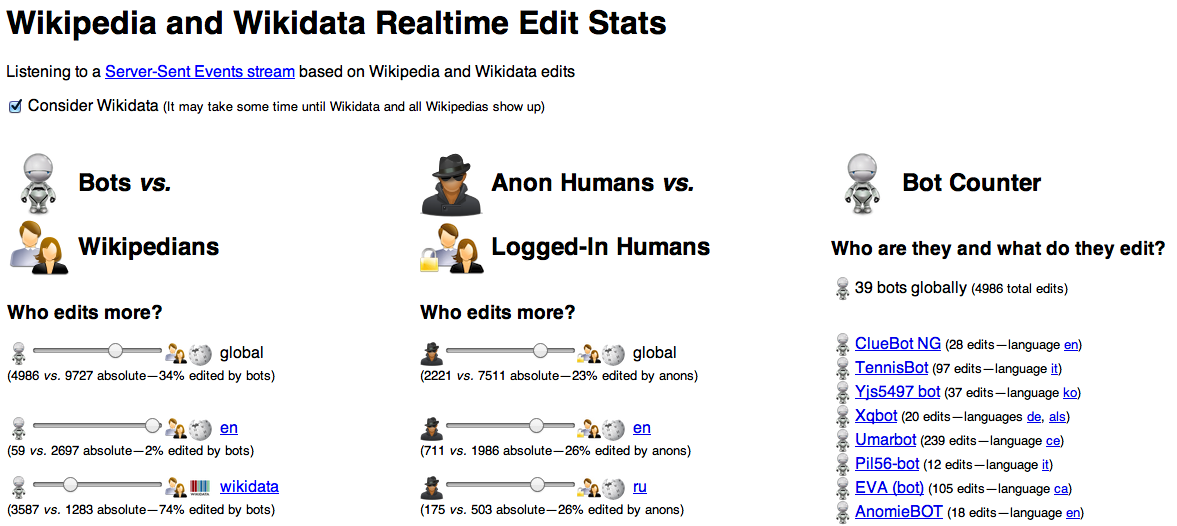
\includegraphics[width=\linewidth]{bots-vs-wikipedians.png}}
  \caption{Screenshot of the application available at \url{http://wikipedia-edits.herokuapp.com/} (cropped)}
  \label{fig:screenshot}
\end{figure*}


\bibliographystyle{abbrv}
\bibliography{references}

\end{document}
